\section{Shared Instruction Cache Design}
\jbs{Akhil in charge.}

\begin{figure}[ht!]
\centering
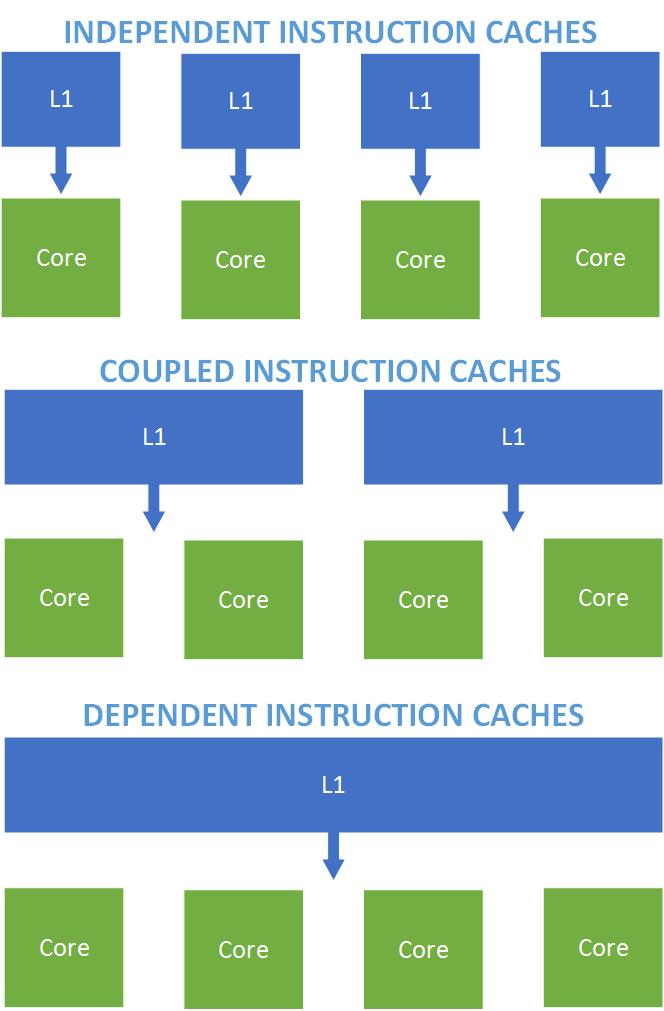
\includegraphics[width=90mm]{graphics/InstructionCacheDesignSketches.jpg}
\caption{(a) Current design of Instruction Caches in an SM, (b) Proposed cache design 1 (b) Proposed cache desgn 2.}
\label{propDesign}
\end{figure}

Most computer architectures build an independent instruction cache for
each processing core.
Reducing the number of instruction caches for the same number of cores
in a multi-core processor has certain advantages. 
First, a shared instruction cache design could reduce the number of
compulsory misses because an instruction previously fetched
by one processor may be available for another processor immediately
rather than requiring an additional cache miss. 
However, the sharing of a single cache among multiple threads will
increase the pressure to that cache, and require additional read ports
for each processor.
\jbs{not sure about the following sentence. It needs justification.}
We hypothesized that sharing an instruction cache would result in
increased efficiency and fewer cache misses. 
Figure~\ref{propDesign} shows a traditional instruction cache
arrangement, the proposed design of sharing an instruction cache over
multiple (but not all) cores on a chip, and the last design extends
that sharing to the logical limit where a \emph{single} instruction
cache to be shared by all the cores on a chip.
 




